\documentclass[12pt, a4paper]{report}

% Pull in the Custom Computing group formatting
\usepackage{ccrep}

% --- Additional packages ---
\usepackage{booktabs}
\usepackage{array}
\usepackage{enumitem}

% --- Referencing (Vancouver Style Mandated) ---
\addbibresource{references.bib}

% --- Document Metadata ---
\title{Portfolio Optimisation with Causal Networks: Interim Report}
\author{Joshua Muthu}
\cid{06048741}
\supervisor{Dr. Ce Guo and Prof. Wayne Luk}
\secondmarker{Prof. Stephen Weston}
\date{June 2026}

\begin{document}

% --- Front Matter ---
\pagenumbering{roman}

\maketitle

\begin{abstract}
\noindent Portfolio optimisation has long relied on correlations between asset returns.
However correlation is undirected, static, and can be spurious.
I investigate whether replacing the correlation-based driver selection in a recent portfolio optimisation framework, 
Hierarchical Sensitivity Parity (HSP), with a causal structure yields higher returns.
I propose a Causal-HSP strategy with a closed feedback loop. First, selecting a portfolio's common drivers by temporal causal discovery
(DYNOTEARS) rather than by cumulative correlation. 
Second, clustering assets in the resulting causal sensitivity space. 
Third, creating a closed feedback loop whereby
out-of-sample performance updates a driver-utility score that affects the next period's selection.

So far, I have completed full backtests over 2007--2024 (top 100 assets from the S\&P 500, 215 monthly rebalances). I use both one-year and two-year windows for fitting causal graphs.
Causal driver selection has a higher risk-adjusted return than
correlation selection at both windows (Sharpe 0.382 versus
0.370--0.371), though this is not statistically significant.
The addition of a closed loop is not robust to the window size: it is
significantly worse than the open-loop variants under the two-year window.
This interim report reviews the
relevant literature, describes the system built to date, and sets out the evaluation methodology
and plan for the remaining work through early September.
\end{abstract}

% Acknowledgements not needed for interim report
% \begin{acknowledgements}
% I would like to thank my supervisors, Dr.\ Ce Guo and Prof.\ Wayne Luk, for their guidance.
% \end{acknowledgements}

\tableofcontents
\clearpage

% --- Main Content ---
\pagenumbering{arabic}

% ============================================================
\chapter{Introduction}
% ============================================================

\section{Context and motivation}

Portfolio optimisation divides capital across assets with the aim of maximising returns and minimising risk. Beginning with Markowitz's mean-variance model \cite{markowitz1952portfolio},
modern portfolio theory decomposes an asset's risk into (i) a systematic part, shared with the
broader market and priced through factor models such as the Capital Asset Pricing Model
\cite{sharpe1964capm} and Arbitrage Pricing Theory \cite{ross1976apt}, and (ii) an
idiosyncratic part that diversification across assets can reduce. These two components ordinarily trade off against each other: 
reducing factor exposure tends to concentrate a portfolio, 
while cross-asset diversification reduces variance but tends to
increase factor exposure.

Mathematically, optimisation methods generally rely on the covariance (or equivalently correlation) matrix of returns. 
However, correlation has several inherent issues.
It is undirected (it cannot define a temporal ordering between assets' movements); it is static (it does not track how market structure shifts during crises); and can be spurious (two assets may be correlated but have no true causal relationship) \cite{simon1954spurious}. 
The last point is particularly problematic:
a variable that simply co-moves with equities (e.g.~an equity index) can be
indistinguishable from a variable that causally drives them. 
In the context of factor investing, spurious correlation manifests as
overfitting and false factor discoveries \cite{lopezdeprado2023causal}.

Causal discovery overcomes these problems by learning from observational data to identify directed, causal relationships between assets.
Recent work has begun to apply causal-discovery algorithms to equity
markets \cite{howard2025causal,tang2024trading}. In addition, methodological advancements, such as the score-based causal structure discovery algorithm NOTEARS \cite{zheng2018notears}, and its time-series extension DYNOTEARS
\cite{pamfil2020dynotears}, have made larger-scale applications of causal discovery more tractable.

This project applies causal discovery methodologies to portfolio optimisation, specifically using a recent optimisation method called Hierarchical Sensitivity Parity (HSP) \cite{rodriguez2023hsp}.
HSP first selects common drivers of assets (such as government bonds, commodity futures, macroeconomic indicators, and FX pairs) via cumulative correlation,
then clusters assets in sensitivity space (i.e.~by the similarity of their sensitivities to a set of common drivers).
I investigate whether replacing HSP's correlation-based driver selection with a causal discovery algorithm
produces more robust portfolios, particularly around regime changes where
correlation-based methods are especially vulnerable. 
I also add a closed feedback loop in which
out-of-sample portfolio performance updates a driver-utility score that shapes the next period's driver selection.
I refer to HSP with causally-selected drivers as Causal-HSP, and to the version with the added
feedback loop as closed-loop Causal-HSP.

\section{Challenges, novel contributions, and quantified benefits}
\label{sec:challenges}

The project is framed around three key technical challenges, my novel contributions to address each one, and the quantified benefits over existing results.

\begin{enumerate}
    \item \textbf{Key technical challenges}
    \begin{enumerate}[label=\textbf{C\arabic*}]
        \item Causal driver identification at portfolio scale. HSP selects drivers by
            cumulative correlation, which conflates co-movement with causation.
            The challenge is to identify genuinely causal drivers instead. 
            This requires causal discovery over a large selection of potential drivers and assets, plus a directional
            prior (drivers cause assets but not vice versa). 
            However, it must also be computationally tractable, and many of the causal discovery algorithms are not readily parallelisable.
            
        \item Using directional causal structures in the context of a symmetric allocation mechanism.
            Hierarchical risk-parity methods cluster on a symmetric distance matrix, but causal
            graphs are directional. Naive symmetrisation of the causal adjacency matrix would discard the directional information that motivates the
            whole approach.
            
        \item Closed-loop feedback implementation.
            I hypothesise that allowing out-of-sample
            performance to feed back into selection should improve robustness across regime changes.
            However, such feedback is not a standard feature of HSP.
            The framework will therefore need to be adjusted to incorporate closed-loop feedback, and I will have to evaluate whether this feedback will indeed improve robustness.
            
    \end{enumerate}

    \item \textbf{Novel contributions to address each of the respective challenges}
    \begin{enumerate}[label=\textbf{A\arabic*}]
        \item I propose a causal factor discovery pipeline. It runs a temporal
              causal-discovery algorithm (DYNOTEARS, with VARLiNGAM as a comparison; see
              Section~\ref{sec:temporal-cd}) over the joint panel of drivers and assets, so drivers
              are chosen by causal evidence rather than correlation. The directional prior is
              enforced by forbidding asset-to-driver edges. To keep discovery tractable, a
              greedy selector prunes the candidate set, the number of drivers is chosen
              based on the data, and the costly calibration step is parallelised across permutations.

        \item I construct portfolios with Causal-HSP, working inside the sensitivity space.
              Each asset's sensitivities to the selected drivers form a Euclidean embedding, so the
              distance matrix is symmetric by construction. Causal information then drives the
              clustering directly, with no symmetrisation of the causal graph, and the allocation
              step is left unchanged from the original HSP.

        \item I extend HSP with a closed feedback loop, which standard HSP lacks. Out-of-sample performance is attributed back to the drivers that shaped the portfolio
              and updates a utility score, which feeds into the next period's selection. I then evaluate whether this feedback improves robustness,
              using a backtest at two window durations.
    \end{enumerate}

    \item \textbf{Quantified benefits over existing published results (preliminary results; see Chapter~\ref{chap:progress})}
    \begin{itemize}
      \item Causal driver selection has a better Sharpe ratio than the cumulative-correlation baseline at
            both windows (0.382 versus 0.370--0.371), and likewise with respect to CAGR (5.07--5.14\% versus
            4.87--4.93\%), net of costs over 215 monthly rebalances, 2007--2024.
            
      \item The causal selector switches between 26 distinct drivers tracking the macro regime, while
            the correlation selector only identifies around half that number every rebalance.
            
      \item Adding the feedback loop is not robust to the window: it is significantly
            worse than the open-loop version at the 504-day window ($\Delta$Sharpe $-0.009$, $p=0.031$).
            
      \item The most closely-related prior work (Howard et al.\ \cite{howard2025causal}), which applies
            DYNOTEARS to the S\&P~500. However, it never sets portfolio weights based on the causal graph; my project is novel in that respect.
            
    \end{itemize}
\end{enumerate}

\section{Report structure}

Chapter~\ref{chap:background} reviews the relevant literature on portfolio optimisation, causal
discovery and the intersection of the two. Chapter~\ref{chap:progress} describes
the system built to date, organised around the above achievements A1 to A3, and reports preliminary results
and the obstacles encountered. Chapter~\ref{chap:plan} discusses the evaluation methodology and the
plan for the remainder of the project.

% ============================================================
\chapter{Background and Related Work}
\label{chap:background}
% ============================================================

\section{Portfolio optimisation}

Modern portfolio theory \cite{markowitz1952portfolio} chooses weights $w$ to minimise portfolio
variance $w^\top \Sigma w$ for a given expected return, where $\Sigma$ denotes the return covariance
matrix. The solution requires inverting $\Sigma$. This is problematic in practice: sample
covariance matrices for large universes of assets are noisy and near-singular, so the optimiser amplifies
estimation error and produces unstable weights that perform poorly out of sample.
Factor models address part of this by attributing returns to a small number of common factors,
each asset carrying a vector of factor sensitivities (betas); CAPM \cite{sharpe1964capm} uses a
single market factor, which Arbitrage Pricing Theory \cite{ross1976apt} generalises to several. 
Under these models, risk splits into a
systematic component, reduced by managing factor exposure, and an idiosyncratic component, reduced
by diversifying across assets.
These two forms of diversification usually trade off against one
another, and reconciling them is a recurring theme in the literature.

\section{Hierarchical Risk Parity}
\label{sec:hrp}

Hierarchical Risk Parity (HRP) \cite{lopezdeprado2016hrp} avoids matrix
inversion entirely. It proceeds in three steps. First, it converts the correlation matrix into a
distance matrix and applies hierarchical (single-linkage) clustering to obtain a dendrogram of the
assets. Second, it quasi-diagonalises the covariance matrix by reordering assets so that
similar assets sit close together, concentrating large covariances near the diagonal. Third, it
allocates capital by recursive bisection: starting from the top of the tree, it splits the
asset set into two clusters, computes each cluster's variance using inverse-variance weights, and
allocates between the two clusters in inverse proportion to their variances, recursing down the
tree. Because it never inverts the covariance matrix, HRP avoids the ill-conditioning that
destabilises mean-variance optimisation, and it outperforms both minimum-variance and
inverse-variance portfolios out of sample \cite{lopezdeprado2016hrp}. For this project,
the clustering step needs only a symmetric, non-negative distance matrix, and the allocation step
needs only cluster variances. The two stages are cleanly separable.

\section{Hierarchical Sensitivity Parity}
\label{sec:hsp}

Hierarchical Sensitivity Parity (HSP) \cite{rodriguez2023hsp} is a recent extension of HRP.
It keeps the framework of clustering followed by bisection, but changes what the assets are clustered on. Instead of clustering on the
correlation of returns, it clusters on the similarity of assets' sensitivities to a set of
common drivers. The motivation is the commonality principle: the optimal drivers of a
portfolio are those that are most frequently and persistently selected across its constituents, both in
terms of persistence over time and probability of being causal. Rodriguez Dominguez
\cite{rodriguez2023hsp,rodriguez2025causal} argues, via the Reichenbach common-cause principle
\cite{hitchcock2020reichenbach}, that if the drivers satisfy the commonality principle then a
conformal map exists between the unconditional return space (where angles between asset vectors
represent correlations) and the sensitivity space (whose coordinates are the common drivers). A
conformal map preserves angles, and therefore correlation and clustering structure. 
As a result, both idiosyncratic
and systematic diversification can be achieved at the same time, escaping the diversification
trade-off described above.

For each asset, HSP trains a feed-forward neural network that maps driver values to the
asset's return, and extracts the sensitivity vector
\(
  s_i = \left( \partial f_i / \partial d_1, \ldots, \partial f_i / \partial d_K \right)
\)
by automatic adjoint differentiation, averaged over the fit window. The sensitivity
distance between assets
\(
  D_{ij} = \lVert s_i - s_j \rVert_2
\)
defines the matrix on which assets are clustered. 
Recursive bisection with sample-variance weights is then used for asset allocation, as in HRP. 
The problem this project targets is that HSP
still selects its common drivers by cumulative correlation with the portfolio
constituents over a window. 
This is the correlation-based selection that the commonality
principle's appeal to causality was meant to move beyond. The author also identifies several open issues, including regimes,
non-stationarity, and overfitting \cite{rodriguez2023hsp}.

\section{Causal discovery}
\label{sec:cd-foundations}

Causal discovery learns directed structure from observational data \cite{spirtes2000causation,kaddour2022causalml}. A structural causal model represents a system as a
directed acyclic graph (DAG) over variables, in which each variable is a function of its parents
and a noise term. A DAG is a Bayesian network for a distribution when the distribution factorises
according to the local Markov condition: each variable is independent of its non-descendants given
its parents. 
Reconstructing DAGs from observational data requires the faithfulness assumption.
This states that if two variables appear statistically independent in the data, then they must be structurally disconnected (d-separated) in the true causal graph.
Constraint-based methods such as PC and FCI \cite{spirtes2000causation} test conditional
independencies to recover the graph, but they scale exponentially in the number of nodes.
They also lean on strong faithfulness, which is fragile in finance: markets
contain many mutually offsetting causal relationships that can leave d-connected pairs of variables with small
marginal correlations, breaking the assumption \cite{howard2025causal}.

Score-based methods avoid invoking faithfulness by searching for the graph that best fits a regularised
score, but the acyclicity constraint is combinatorial and therefore computationally challenging. 
NOTEARS \cite{zheng2018notears} reformulated acyclicity as a smooth, continuous equality constraint,
\(
  h(W) = \operatorname{tr}\!\big(e^{\,W \circ W}\big) - d = 0,
\)
where $W$ is the weighted adjacency matrix, $\circ$ is the Hadamard product and $d$ the number of
nodes. This turned structure learning into a continuous optimisation problem solvable with standard
solvers, and made score-based discovery tractable at scale. 

The LiNGAM framework
\cite{shimizu2006lingam} takes a different route, exploiting the non-Gaussianity of the noise
to identify a unique causal ordering without needing prior structure. 
This is well-suited to
financial returns, which are generally heavy-tailed and non-Gaussian.

For these reasons, I use the
NOTEARS and LiNGAM families of causal discovery algorithms in this project \cite{kaddour2022causalml,silva_causalinf}.

\section{Temporal causal discovery}
\label{sec:temporal-cd}

Asset returns are time series, so I use dynamic Bayesian networks, which add lagged
variables to the causal graph.
Edges split into intra-slice edges $W$ (capturing contemporaneous
relationships at time $t$) and inter-slice edges $A_1, \ldots, A_P$ (capturing lagged
relationships from $t-p$ to $t$).
In econometric terms, this is equivalent to a structural vector autoregression (SVAR),
\begin{equation}
  X = X W + \sum_{p=1}^{P} Y_p A_p + Z,
\end{equation}
where $X$ is the $n \times d$ panel, $Y_p$ are its lags, and $Z$ is noise. The acyclicity
constraint applies only to $W$, because the lagged edges point forward in time and cannot create
cycles.

DYNOTEARS \cite{pamfil2020dynotears} applies the NOTEARS smoothed acyclicality constraint to this SVAR, minimising a penalised least-squares loss
\(
  \tfrac{1}{2n}\lVert X - XW - \sum_p Y_p A_p\rVert_F^2
  + \lambda_W \lVert W\rVert_1 + \lambda_A \sum_p \lVert A_p\rVert_1
\)
subject to $h(W)=0$. I use it as the primary causal discovery method in my project: it is score-based (no faithfulness assumption), it scales to high dimension, and specific edges can be forbidden (which
is required for enforcing the directional prior as in C1).

VARLiNGAM \cite{hyvarinen2010varlingam} estimates an SVAR by taking the (non-Gaussian) residuals of a standard reduced-form autoregression, applying independent component analysis, and thereby uncovering a DAG that orders the instantaneous causal effects.
Because the non-Gaussian assumption matches the empirical distribution of financial returns, 
and because causal ordering can reflect underlying regime changes, it is retained as a robustness comparison to DYNOTEARS.

NTS-NOTEARS \cite{sun2023ntsnotears} replaces linear relationships between nodes in the causal graph with 1D convolutional networks, which allows for non-linear causal relationships.
Time allowing, it would be an insightful extension, as it would unify causal discovery and sensitivity extraction in a single model.

\section{Causal methods in quantitative finance}
\label{sec:cd-finance}

The closest existing work is Howard, Lohre and Mudde \cite{howard2025causal}, who apply DYNOTEARS
to the S\&P~500 and build three investment use-cases on the discovered networks: 
peer groups for factor neutralisation, 
a low-centrality factor (long causally peripheral, short causally central
stocks), 
and a market-timing indicator based on changes in network density. 
Their conclusion is
that causal networks complement rather than consistently beat correlation-based methods: 
they sometimes raise risk-adjusted returns through better stock selection, but they are computationally intensive and hard to interpret. 
Two of their findings are particularly relevant for this project. 
First, they find the inter-slice (lagged)
weights to be almost always negligible for daily and monthly returns, so the contemporaneous block
dominates. 
This is evidence for retaining VARLiNGAM, which models lags and non-Gaussianity explicitly, as a check. 
Second, they never use the causal graph to set portfolio
weights directly. Their causal graph is mapped to an embedding space, which is then clustered into peer groups.
By contrast, this project directly converts causal structure into portfolio allocation.

Other recent work confirms both the promise and the practical difficulty of applying causal discovery to finance. 
Tang \cite{tang2024trading}
designs trading strategies from time-series causal-discovery output (including from VARLiNGAM) on Chinese and US markets, finding profitable signals but identifying computational cost and
scalability binding constraints. 

\section{Research gap}
\label{sec:gap}

Table~\ref{tab:gap} compares this project to previous research.
The proposed closed-loop Causal-HSP method fills all three gaps at once: it selects drivers
causally (C1), unlike HSP's correlation-based selector \cite{rodriguez2023hsp}; it routes that directional information into a symmetric allocator through the
sensitivity space (C2), unlike Howard et al.'s embedding clustering \cite{howard2025causal}; and it creates a closed feedback loop in which realised portfolio performance affects subsequent driver selection (C3).

\begin{table}[t]
  \centering
  \caption{Positioning of this work against the closest related approaches.}
  \label{tab:gap}
  \begin{tabular}{l c c c c}
    \toprule
    Approach & Driver selection & Directional & Weights from & Performance \\
             &                  & structure   & graph        & feedback \\
    \midrule
    HRP \cite{lopezdeprado2016hrp}        & none (correlation) & no  & n/a & no \\
    HSP \cite{rodriguez2023hsp}           & cumulative corr.   & no  & yes & no \\
    Howard et al.\ \cite{howard2025causal} & causal (DYNOTEARS) & yes & no  & no \\
    \textbf{This work}                    & \textbf{causal}    & \textbf{yes} & \textbf{yes} & \textbf{yes} \\
    \bottomrule
  \end{tabular}
\end{table}

% ============================================================
\chapter{Technical Achievements and Progress}
\label{chap:progress}
% ============================================================

This chapter describes the system built to date, organised around the three achievements A1--A3
outlined in Section~\ref{sec:challenges}, and then reports preliminary results and the obstacles
encountered. 
As of this interim report, the main experiments are complete: a first full backtest has already been completed.

\section{System overview}
\label{sec:overview}

The pipeline consists of two stages that run at each monthly rebalance date $t$.

Stage~1 runs causal discovery on the joint panel $X = [\,D \mid A\,]$ of drivers and assets
over the window (A1), then selects the top $K$ drivers based on their causal influence plus their
historical utility (from the feedback loop). Then, for each asset, the sensitivity matrix $S$ is extracted by feed-forward network plus
automatic adjoint differentiation.

Stage~2 forms the sensitivity distance matrix
$D_{ij} = \lVert s_i - s_j \rVert_2$, clusters and allocates by recursive bisection with
sample-covariance variances (A2). 
Then, it uses the allocated weights for the next month and feeds the resulting out-of-sample
reward back into driver utility for the next rebalance (A3) (Section~\ref{sec:a3}).

I compare four variants, which isolate the effect of each design choice:
\begin{itemize}[itemsep=1pt, topsep=3pt]
  \item V0 (baseline): standard HSP; drivers selected by cumulative correlation; no feedback.
  \item V1: Causal-HSP; drivers selected by causal discovery; no feedback (open loop).
  \item V2: closed-loop Causal-HSP; V1 plus the closed feedback loop (the full proposed method).
  \item V0$'$: Causal-HRP; but only clustering on asset-to-asset causal
        structure, with no drivers. This tests whether the exogenous drivers add value.
\end{itemize}

\section{A1: causal factor discovery (Stage 1)}
\label{sec:a1}

Running the intended large number of experiments on the full S\&P~500 proved too computationally intensive. 
I therefore planned to use the S\&P~100, however I was unable to find a full historical list of its components.
I therefore reconstruct approximate S\&P~100
membership by taking, at each rebalance, the top 100 constituents by market
capitalisation from historical S\&P~500 membership; prices and
historical shares outstanding come from WRDS/CRSP
with a small Yahoo Finance fallback for the most recent days. 
The driver pool comprises 30 to 50
plausibly exogenous macroeconomic and financial series from FRED and Yahoo Finance (rates, credit
spreads, commodities, FX, volatility indices, international equity).
I excluded equity baskets like sector ETFs and US index returns because they are not credibly exogenous.
Series are made stationary by appropriate transforms (e.g.~logarithms and differences) within each window.

I primarily use DYNOTEARS \cite{pamfil2020dynotears} on a rolling basis for causal discovery. The directional
prior of C1, that drivers cause assets and not the reverse, is enforced by forbidding
asset-to-driver edges, which sets the
corresponding entries of $W$ and the $A_p$ to zero.
VARLiNGAM \cite{hyvarinen2010varlingam} is available as a robustness comparator.

Driver selection is a two-step greedy procedure. First, a prune step scores each candidate by its
aggregate lagged outgoing influence on the assets, and keeps a shortlist. 
Then, a greedy-refinement step adds drivers to the selected set by their marginal gain in held-out predictive likelihood. 
The number of drivers $K$ is
not fixed a priori but calibrated by two methods in parallel: the Kneedle
algorithm \cite{satopaa2011kneedle}, which finds the elbow in the sorted causal-score curve, and a
permutation null with Benjamini-Hochberg false-discovery-rate control \cite{benjamini1995fdr}, which counts
how many drivers clear significance. 
However, at the dimensions tested, the
permutation test returns zero significant drivers at the 5\% level, so the operational selector is
always given by the Kneedle elbow (which scales reasonably with universe size, from 9 drivers at $d=65$ to 14
at $d=134$).

\section{A2: Causal-HSP in sensitivity space (Stage 2, open loop)}
\label{sec:a2}

Achievement A2 resolves C2. Rather than symmetrising the directional causal graph, the pipeline
computes per-asset sensitivities of returns to the causally-selected drivers via a feed-forward
neural network and automatic adjoint differentiation, as in HSP (Section~\ref{sec:hsp}).
However, unlike HSP, it does so on a
causally-selected, rather than correlation-selected, driver set. The resulting sensitivity vectors are
in a Euclidean space, so the distance matrix $D_{ij} = \lVert s_i - s_j \rVert_2$ is symmetric by
construction. 
Thus, no symmetrisation of an asymmetric adjacency is ever required, and the directional
information is preserved in how it shaped the selected drivers and their sensitivities. 
The allocation step (recursive bisection with sample covariance) remains the same as in HSP.
This open-loop construction underpins V0, V1 and V0$'$ (Section~\ref{sec:overview}).

\section{A3: closing the loop (feedback)}
\label{sec:a3}

Achievement A3 resolves C3. After holding the weights $w[t]$ for the month, the realised reward is
the excess Sharpe ratio relative to an equal-weight portfolio over the same holding period,
\begin{equation}
  R[t] = \text{Sharpe}\big(\text{portfolio over } [t, t{+}h]\big)
       - \text{Sharpe}\big(\tfrac{1}{N} \text{ over } [t, t{+}h]\big).
\end{equation}
This excess form controls for market-wide regime effects, so drivers are not punished for a crash
that affected everything. 
Reward is attributed to drivers in proportion to how strongly each shaped the
portfolio, via a sensitivity-weighted credit that preserves the total reward,
\begin{equation}
  \text{credit}_d[t] = R[t]\,\frac{\text{influence}_d}{\sum_{d'} \text{influence}_{d'}},
  \qquad
  \text{influence}_d = \sum_i \big| w_i[t]\, s_{i,d}[t] \big|.
\end{equation}
Each selected driver's utility is then updated by an exponential moving average. 
The selector at the next rebalance combines causal evidence and accumulated utility:
\begin{equation}
  U_d[t] = \gamma\, \text{credit}_d[t] + (1-\gamma)\, U_d[t-1],
  \qquad
  \text{score}_d[t] = \alpha\, z\big(\text{causal}_d[t]\big) + (1-\alpha)\, z\big(U_d[t-1]\big).
\end{equation}
Here, $\gamma$ affects the utility's memory and $\alpha$ weights causal evidence ($\alpha = 1$ recovers
the open-loop V1) with history. The full closed-loop method is variant V2.

\section{Preliminary results}
\label{sec:results}

The main experiment ran V0, V1 and V2 over the full 2007--2024 sample (99 assets, 33 driver candidates,
$K=17$ calibrated once, 215 monthly rebalances), at two windows (252 and
504 trading days) as a robustness check, net of 5~bps one-way transaction costs.
Table~\ref{tab:phasei} gives the key metrics, and Table~\ref{tab:sig} gives the significance of the
pairwise differences, assessed by a Politis-Romano stationary block bootstrap
\cite{politis1994stationary} with 2000 resamples.
Figure~\ref{fig:nav} plots the net asset value (NAV)
trajectories, net of cost, over the full sample. Figure~\ref{fig:bars} displays the Sharpe comparisons and the performance over specific regimes such as the GFC and COVID.

\begin{figure}[tbp]
  \centering
  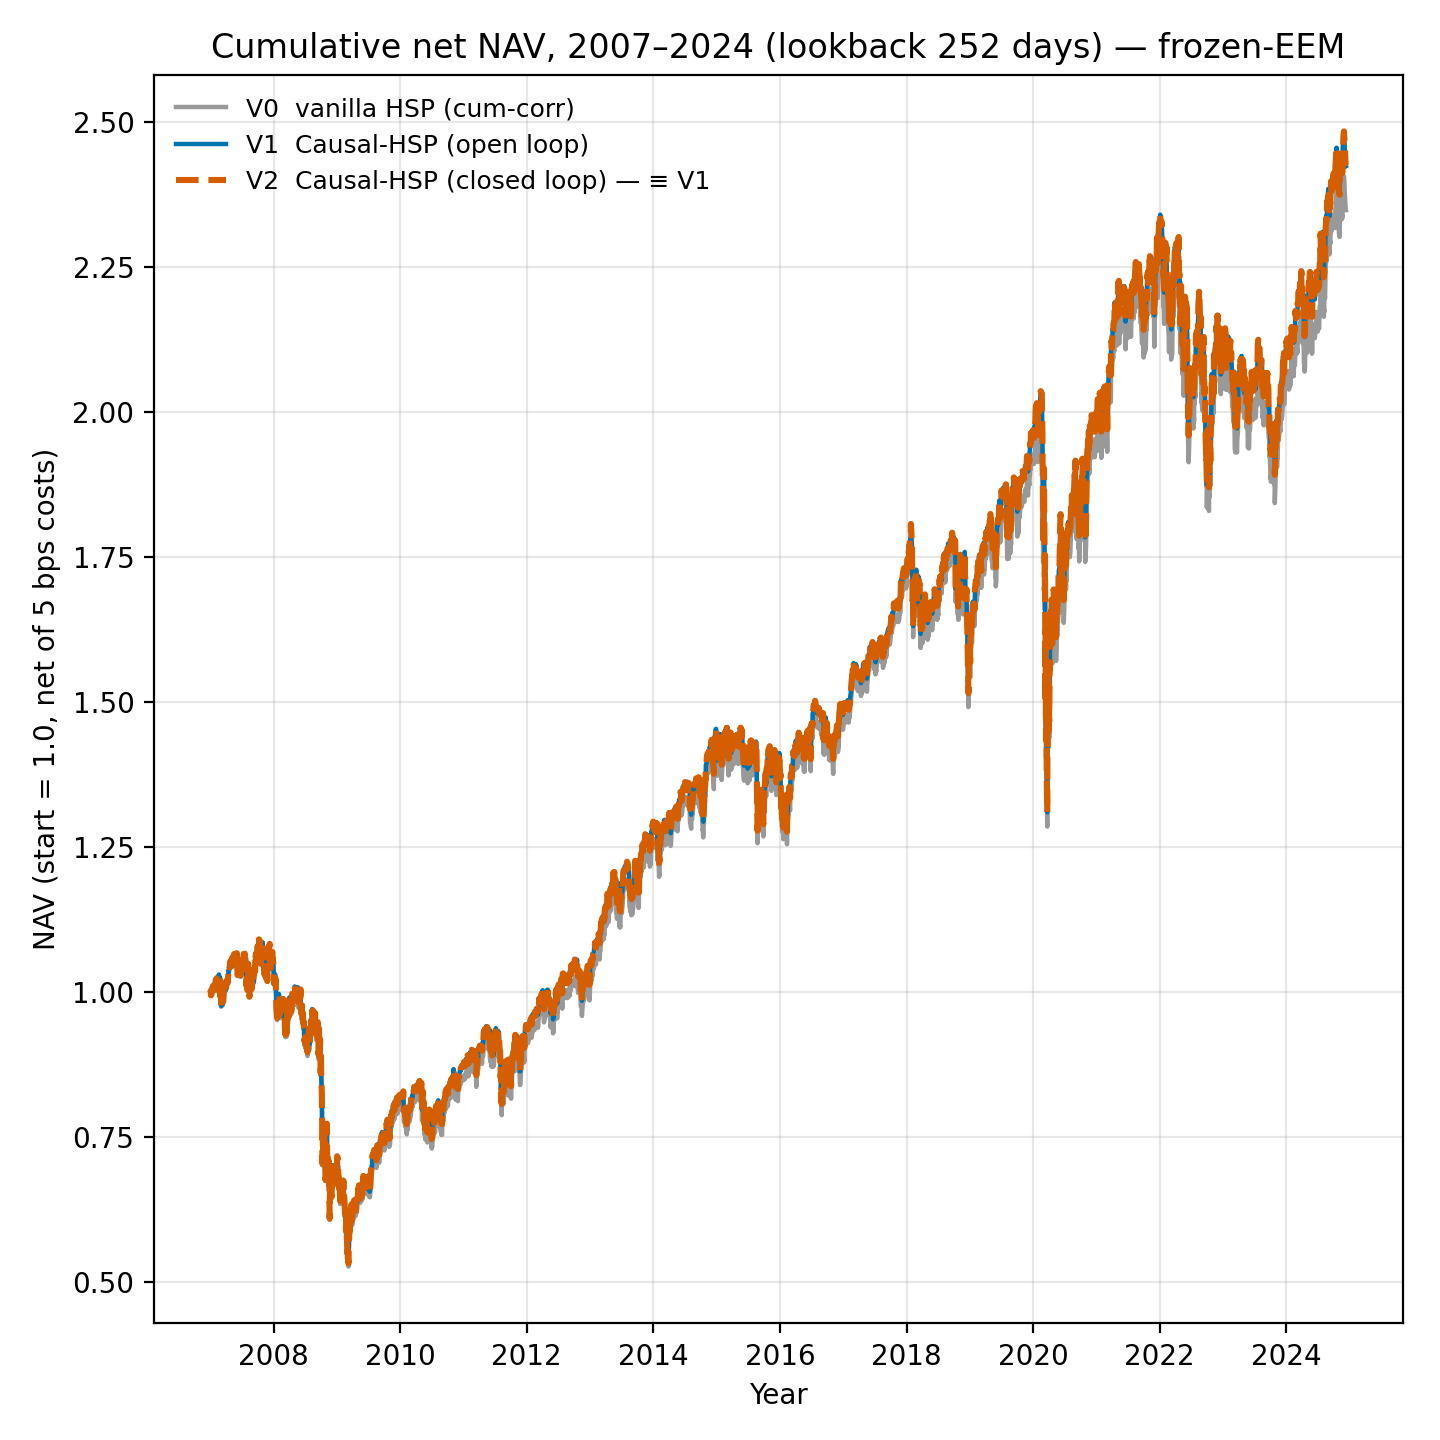
\includegraphics[width=0.76\textwidth]{figures/nav_curve.png}
  \caption{Cumulative net-of-cost NAV for the three variants over 2007--2024 at the 252-day
           window. The causal variants (V1, V2) sit modestly above the correlation baseline
           (V0), the gap widening from around 2018.}
  \label{fig:nav}
\end{figure}

\begin{table}[t]
  \centering
  \caption{Preliminary full-sample results, 2007--2024, net of costs, at two windows.}
  \vspace{0.5em}
  \label{tab:phasei}
  \begin{tabular}{l ccc c ccc}
    \toprule
    & \multicolumn{3}{c}{Window 252 days} & & \multicolumn{3}{c}{Window 504 days} \\
    \cmidrule(lr){2-4} \cmidrule(lr){6-8}
    Variant & CAGR & Sharpe & MaxDD & & CAGR & Sharpe & MaxDD \\
    \midrule
    V0 (cumulative corr.) & 4.87\% & 0.371 & $-51.7\%$ & & 4.93\% & 0.370 & $-51.7\%$ \\
    V1 (causal, open loop)      & 5.07\% & \textbf{0.382} & $-51.2\%$ & & 5.14\% & \textbf{0.382} & $-51.2\%$ \\
    V2 (causal, closed loop)    & 5.07\% & 0.382 & $-51.4\%$ & & 4.97\% & 0.373 & $-51.4\%$ \\
    \bottomrule
  \end{tabular}
\end{table}

\begin{table}[t]
  \centering
  \caption{Significance of pairwise Sharpe differences (Politis-Romano block bootstrap), and
           mean monthly excess-Sharpe edge of V2 over V1 in the 2018Q4 regime-break window.}
  \vspace{0.5em}
  \label{tab:sig}
  \begin{tabular}{l cc}
    \toprule
    Comparison & Window 252 & Window 504 \\
    \midrule
    V1 $-$ V0, $\Delta$Sharpe ($p$) & $+0.011$ ($p=0.19$) & $+0.012$ ($p=0.23$) \\
    V2 $-$ V1, $\Delta$Sharpe ($p$) & $+0.000$ ($p=0.97$) & $\mathbf{-0.009}$ ($\mathbf{p=0.031}$) \\
    2018Q4 regime-break (V2 $-$ V1) & $+0.120$ & $-0.111$ \\
    \bottomrule
  \end{tabular}
\end{table}

\begin{figure}[tbp]
  \centering
  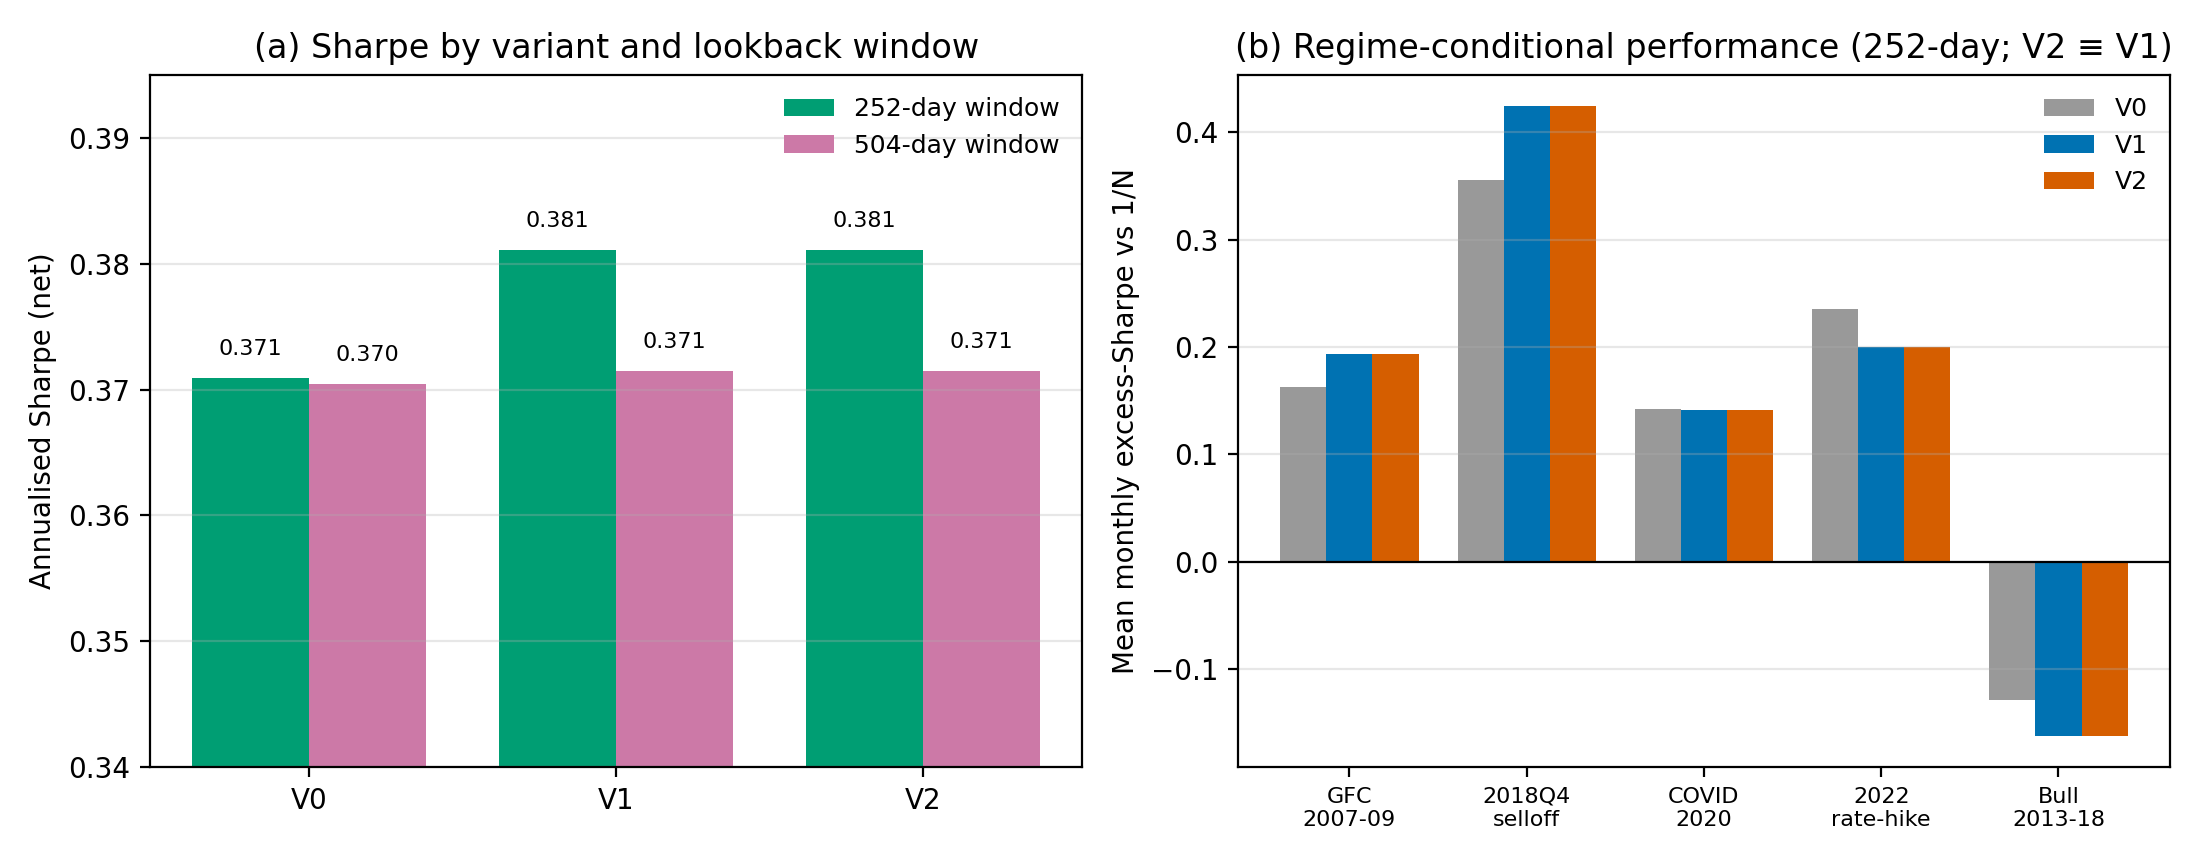
\includegraphics[width=0.92\textwidth]{figures/sharpe_and_regime.png}
  \caption{(a) Annualised net Sharpe by variant at each window: V1 is stable and highest
           at both windows, whereas V2 underperforms at the 504-day window. (b) Regime-conditional mean monthly excess-Sharpe versus equal-weight portfolio
           at the 252-day window: the causal variants outperform the correlational V0 most in stress regimes.}
  \label{fig:bars}
\end{figure}

Three findings stand out.

\begin{enumerate}
  \item V1 beats V0 on
        Sharpe and CAGR at both windows, with the same sign and magnitude
        ($\Delta$Sharpe $\approx +0.011$ to $+0.012$). However, the edge is statistically insignificant over an 18-year sample ($p \approx 0.19$ to $0.23$). The project's primary claim, that causal-discovery driver selection beats
        cumulative-correlation selection, is qualitatively supported.
        
  \item V0 selects essentially the same fixed set of 10 to 14 drivers every rebalance,
        largely international equity indices and the rates curve, because these trivially
        co-move with US equity. 
        By contrast, V1's causal selector rotates across 26 unique drivers,
        tracking the macro regime (rates and credit before COVID, crude and credit at the April
        2020 crash, safe-haven assets mid-crisis, volatility and rates in the recovery). 
        This clearly demonstrates the advantages of causal driver selection over correlation.
        
  \item At the 252-day window, V2
        is roughly neutral overall, with an apparent edge in the 2018Q4 regime break ($+0.120$); but
        at 504 days V2 is significantly worse than open-loop V1 ($p=0.031$) and the 2018Q4
        edge flips sign to $-0.111$. The apparent regime-break benefit is therefore not robust to different window sizes. 
        A plausible explanation is that at 504 days the
        two-year discovery window already yields stable causal graphs, so the utility feedback merely adds noise.
\end{enumerate}

The two-window robustness check exposed the closed loop's fragility (visible in
Figure~\ref{fig:bars}a, where V2 alone drops at the 504-day window). 

% ============================================================
\chapter{Project Plan and Evaluation}
\label{chap:plan}
% ============================================================

\section{Evaluation methodology}
\label{sec:eval}

Every strategy is evaluated using the same backtest: an approximate S\&P~100 universe with
monthly rebalancing over 2007--2024. 
Transaction costs of 5~bps per unit of turnover are charged, with robustness sweeps over $\{0, 5, 10, 20\}$~bps.
Results are reported both gross and net of these costs.

For each strategy, I report risk-adjusted returns, drawdown, total return, risk, concentration, one-way annualised turnover, and the
certainty-equivalent return at risk-aversion levels $\gamma_{\text{RA}} \in \{1, 3, 5\}$, with the
headline at $\gamma_{\text{RA}} = 3$.

I compare my strategies to the following portfolios: an equal-weight ($1/N$) portfolio,
minimum-variance and Markowitz mean-variance portfolios,
standard HRP \cite{lopezdeprado2016hrp}, standard HSP (which is V0) \cite{rodriguez2023hsp}, and the
cap-weighted index for absolute interpretation.

For statistical testing, I take the differences in Sharpe ratio against the V0 baseline are tested with
a Politis-Romano stationary block bootstrap \cite{politis1994stationary} giving 95\% confidence
intervals, as used for the preliminary results in Section~\ref{sec:results}.

I also analyse the performance of the porfolio variances in different regimes. I compute Sharpe, drawdown and turnover within regimes, which are defined in three ways: NBER recession dates, top-versus-bottom VIX quintiles, and
causal-network-density regimes constructed from the discovery output in the manner of
Howard et al.\ \cite{howard2025causal}.

\section{Challenges, achievements and remaining work}
\label{sec:map}

\begin{description}
  \item[A1/C1] Causal factor discovery: this has been built and validated. I need to test whether removing the
        directional prior changes the discovered driver-to-asset structure, to quantify the prior's importance. I also need to test the other causal discovery algorithms (VARLiNGAM and, time permitting, NTS-NOTEARS).
  \item[A2/C2] Using directional causal structures in the context of a symmetric allocation mechanism: this has been completed, bar V0$'$ (the asset-only contol).
  \item[A3/C3] Closed-loop feedback implementation: this has been built and run at two windows. 
  However, I need to implement closed-loop feedback for VARLiNGAM and NTS-NOTEARS. I also need to conduct a hyperparameter sweep over $\alpha$, $\gamma$, and $K$.
\end{description}

\section{Timeline}
\label{sec:timeline}

\begin{description}
  \item[Phase 1 (Now to 31 July).] Run the directional-prior verification; run VARLiNGAM as a comparator; run the V0$'$ asset-only variant; sweep $\alpha$, $\gamma$, and $K$. 
  Time permitting, employ NTS-NOTEARS in the causal driver selection step too.
  \item[Phase 2 (1 August to 9 September).] Writing and polishing the final report.
\end{description}

\section{Ethical considerations}
\label{sec:ethics}

No ethical considerations have been identified for this project.

% ============================================================
\chapter{Summary and Outlook}
\label{chap:conclusion}
% ============================================================

This project investigates whether causal structure, rather than correlation, makes for more robust
portfolio diversification. 
The proposed closed-loop Causal-HSP strategy first selects a portfolio's common drivers
by temporal causal discovery under a directional prior (A1, addressing C1).
Second, it constructs portfolios
in the resulting causal sensitivity space,
so that directional information can be used in an allocation step (that requires symmetric matrices) without being discarded (A2, addressing C2).
Third, it closes a feedback loop in
which realised performance shapes the next period's selection of drivers (A3, addressing C3).

As of the time of writing this interim report, the main system is built and a first full backtest (2007--2024, two windows) is
complete. There are two key preliminary findings: first, causal driver
selection beats cumulative-correlation selection on risk-adjusted return at both one-year and two-year windows
(Sharpe 0.382 versus 0.370--0.371), though the edge is not statistically significant;
and second, the closed-loop extension is not robust to the window. The
remaining work, set out in Chapter~\ref{chap:plan}, is chiefly robustness work, implementing additional causal discovery algorithms, and writing.

% ============================================================
% --- Back Matter ---
% ============================================================
\clearpage
\printbibliography[heading=bibintoc, title={References}]

\chapter*{Declarations}
\addcontentsline{toc}{chapter}{Declarations}
This report is my own work. The
research was conducted under the supervision of Dr.\ Ce Guo and Prof.\ Wayne Luk. Generative AI (Anthropic's Claude) was used to assist with drafting and proofreading the prose of this
report and as a coding assistant during implementation; all technical content, design decisions,
experiments and results are my own, and all AI-assisted text was reviewed and edited by me.

\end{document}